% !TeX spellcheck = de_DE
%%% Ne pas modifier jusqu'à la ligne 25
\documentclass[a4paper,14pt,UTF8]{article}
\usepackage[utf8]{inputenc}
% \usepackage[french]{babel}
\usepackage[left=2cm,right=2cm,top=3cm,bottom=2cm, headheight=1.5cm,headsep=1.5cm]{geometry}

\usepackage{palatino}
\usepackage{setspace}
\usepackage{caption}
\usepackage{float}%控制浮动体位置
%设置段落之间的距离,若不需要删除或者注释掉即可。
\usepackage{blindtext}
\usepackage{fancyhdr}
\usepackage{xcolor} % 代码高亮

\usepackage{mathrsfs}
\usepackage{amsmath,amsfonts,amssymb,dsfont}
\usepackage{graphicx}
\usepackage{enumitem}		%\enumerate-resume
\usepackage[colorlinks=true,unicode={true},hyperindex=false, linkcolor=black, urlcolor=black]{hyperref}
\usepackage{lastpage} 
\usepackage{ctex}			% 中文
\usepackage{comment}		% 注释大段代码

%\renewcommand\thesection{\Roman{section}~-~}
%\renewcommand\thesubsection{\Roman{section}.\Alph{subsection}~-~}
%\renewcommand\thesubsubsection{\Roman{section}.\Alph{subsection}.\arabic{subsubsection}~-~}
\renewcommand\thesection{\arabic {section}}


\setcounter{secnumdepth}{3}
\parindent=0pt

\usepackage{fancyhdr}
\pagestyle{fancy}

\lhead{SJTU-ParisTech}
%%%%%%%%%%%%%%%%%%%%%%%%%%%%%%%
\chead{Hadoop MapReduce "from scratch" on Java}
\rhead{page \thepage\ of \pageref{LastPage}} % 当前页 of 总页数

\begin{document}
	
	\renewcommand{\labelitemi}{$\blacktriangleright$}
	\renewcommand{\labelitemii}{$\bullet$}
	
	\linespread{1.15}
	\selectfont
	\setlength{\parskip}{0.5em}
	
	
	%%% Page de garde
	\thispagestyle{empty}
	\begin{center}
		
\includegraphics{cover5}
		\hspace{60pt}
		
\includegraphics{cover2}
	\end{center}
	%
	\vspace{125pt}
	%
	\begin{center}
		\scalebox{1.3}{\LARGE{\textbf{Project2: Hadoop MapReduce "from scratch" }}}
	\end{center}
	%
	\vspace{2em} \Large
	%
	\begin{center}
		\textbf{褚子豪 \quad 516260910011 \\ 邓若凡 \quad 516261910008 \\ 王甫 \qquad 516261910014}

	\end{center}
	%
	\vspace{1em}
	%
	\begin{center}
		
\includegraphics[scale=1.2]{cover3}
	\end{center}
	%
	\vspace{1em} \normalsize
	%

	
	\newpage
	\begin{center}
		\tableofcontents
	\end{center}
	\numberwithin{equation}{section}
	\clearpage
	
	
	\section{System diagram}
	\quad The overall MapReduce word count process is almost the same as presented in the Project2 presentation slides, but there are still some differences. We have used docker to realize the slaves. The system diagram of our program design is as following:
	
	\begin{figure}[h]
		\setlength{\abovecaptionskip}{-0.cm}
		
	\begin{center}
		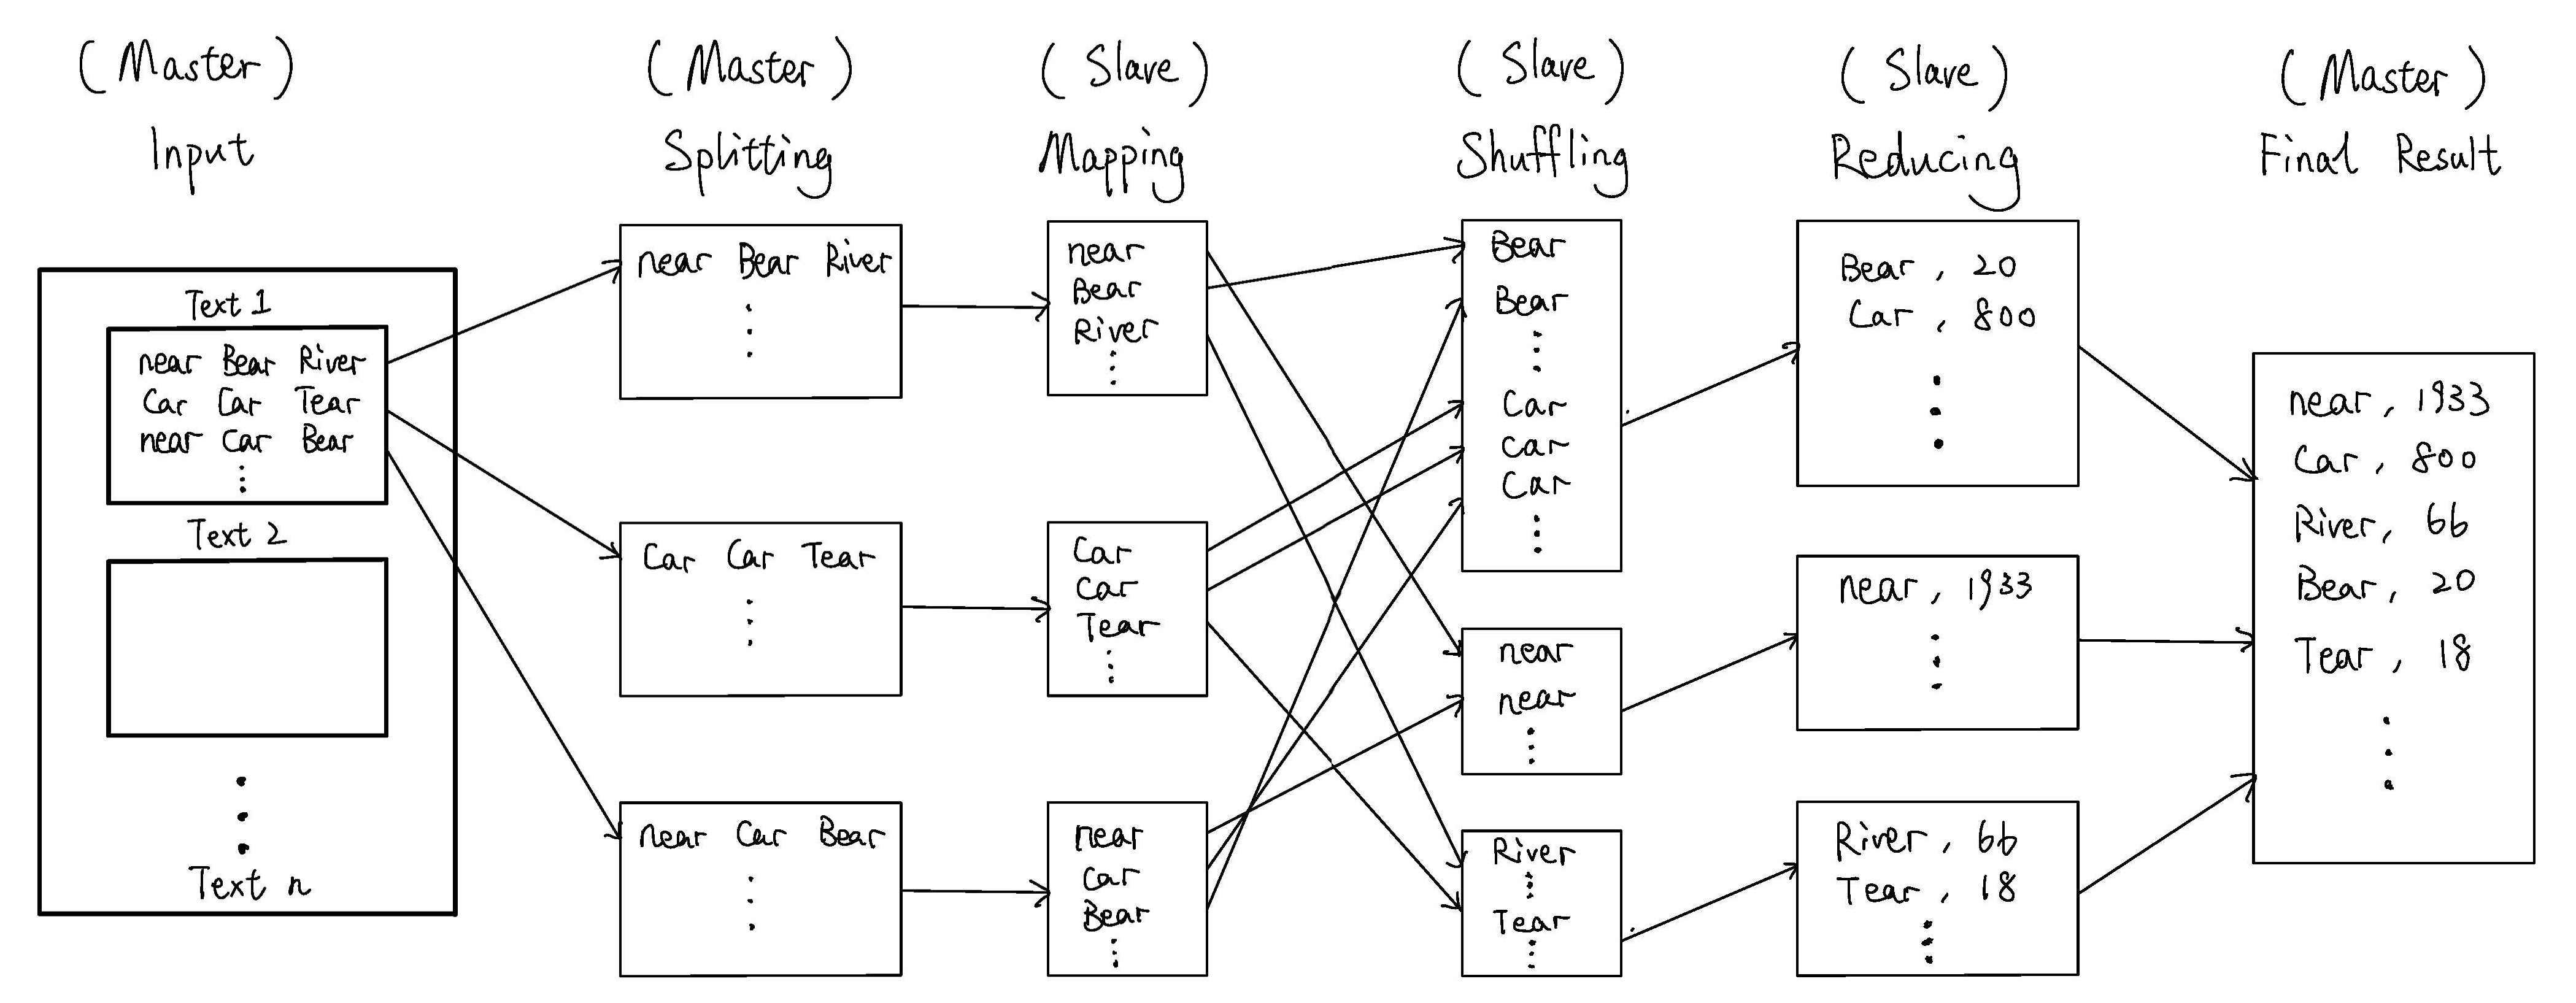
\includegraphics[width=17cm]{system_diagram}
	\end{center}
		\caption{System diagram of the program}
	\end{figure}
	

	\section{Functions description}
	
	\subsection{\textit{BASIC.java}}
	\quad The aim of the file \textit{BASIC.java} realizes the trivial method of word counting on one processor. Generally speaking, it reads files in a folder, splits the words contained, counts the number of occurence of the words and realizes a quick sort according to frequency and letter priority.\par 

	\begin{itemize}
	\item 
	Function \textit{readFile} is designed to read all the files in a folder and split the words contained. Then use a HashMap to store the number of occurence attached to each word appeared.\\
	
	\item
	Function \textit{wordCmp} is used for comparing priority of two words. The first criteria is the number of occurence while the second one is the name of the word. If data[i] has higher priority compared with data[j], then return true.\\
	
	\item
	Function \textit{partition} is a mono-direction partition from left to right which put the words with a higher priority to the left side of the pivot and those with a lower priority to the right side.\\
	
	\item
	Function \textit{sort} realizes a quick sort without recursion by using stack. Function \textit{wordCmp} and Function \textit{partition} are also called to realize the quick sort algorithm.\\

	\item
	Function \textit{output} writes all the words and corresponding frequencies into a file to store them. \\	
	\end{itemize}
	
		  
	\subsection{\textit{MASTER.java}}
	\quad The file \textit{MASTER.java} defines the actions in the master program. In our design, master is called twice, one for the first step: splitting and distributing while the other for the last step: gathering and final sorting. \par 

	
	\begin{itemize}
		
		\item 
		Function \textit{distribute} is designed to read all the files in the folder and divide them into three files (Sx1, Sx2, Sx3) then distribute to the three slaves. \\
		
		\item
		Function \textit{collect} is used to gather the files already reduced by the slaves (RM1, RM2, RM3) and store the results for sorting.\\
		
		\item 
		Functions \textit{partition} , \textit{wordCmp} and \textit{output} are the same as those in BASIC.java.	\\	
		
		\item 
		Function \textit{sort} realizes a quick sort using the files gathered by Function \textit{collect} and obtain the final results \textit{result.txt}.
		
	\end{itemize}

     
	\subsection{\textit{SLAVE.java}}
	
	\quad The file \textit{SLAVE.java} defines the actions in the slave program. We have created three slaves using docker. Each one is responsible for Mapping, Shuffling and Reducing work with the files it receives. In our design, each slave is called twice, first time for mapping and transfering while the second time for reducing.\par

	
	\begin{itemize}
		
		\item 
		Function \textit{map} is designed to allocate the words by the beginning lettre. We use the first letter "R" and "i" to divide the words on a slave into three parts and store them respectively into three files. \\
		
		\item
		Function \textit{transferSM} sends the files obtained by Function  \textit{map} to the corresponding slave. For example, on slave 1, we have the original file received Sx1. We divide it into SM11, SM21, SM31 in the previous function, then send SM11 to itself, SM21 to slave2 and SM31 to slave3.  \\
		
		\item
		Function \textit{reduceSM} is used for reducing the files obtained on a slave after mapping. For example, for slave1, it receives the files SM11, SM12, SM13 from itself, slave2 and slave3. Then it count the frequency of the words contained in these files (reducing) and store them in the file RM1. \\
		
	\end{itemize}
	  
	\section{How to build/run}
	
	\subsection{Preamble}
	
	\quad Our program should be run on Linux. Docker and Java environment are needed. There are also some preparation works: 

	\begin{flushleft}
	
		$\bullet$ \ Use docker to create three containers with names: worker1, worker2 and worker3. Don't need to run them in advance, all the implementations are written in \textit{deploy.sh}. \par
		
		$\bullet$ \ Create a virtual network and confirm that all the three containers are connected. \par
		
		$\bullet$ \ Try to transfer files between containers using scp service (ex. Hello.txt). Just to avoid the confirmation of transmission when we run the program. \par
		
		$\bullet$ \ Type a command in the shell using sudo and put in the password. Just to avoid entering the password later. \par
	
	\end{flushleft}	
	
	\subsection{Build and Run}
		\quad All the instructions have been written in the file \textit{deploy.sh}, including the start of containers, implementation of master and slaves, file transmission between the master and slaves, and timing. We firstly compile the three Java files then test  them  using the following commands: 
	\begin{flushleft}
		
		$\bullet$ \ Use "\textit{sh deploy.sh compile}" to compile the three .java files into runnable jars. \par
		
		$\bullet$ \ Use "\textit{sh deploy.sh basic \#foldername}" to test the trivial method. The result is stored in \textit{result.txt}. \par

		$\bullet$ \ Use "\textit{sh deploy.sh master \#foldername}" to test the MapReduce method. The result is stored in \textit{result.txt}.\par

	\end{flushleft}
	
	\begin{figure}[h]
		\setlength{\abovecaptionskip}{-0.cm}
		
		\begin{center}
			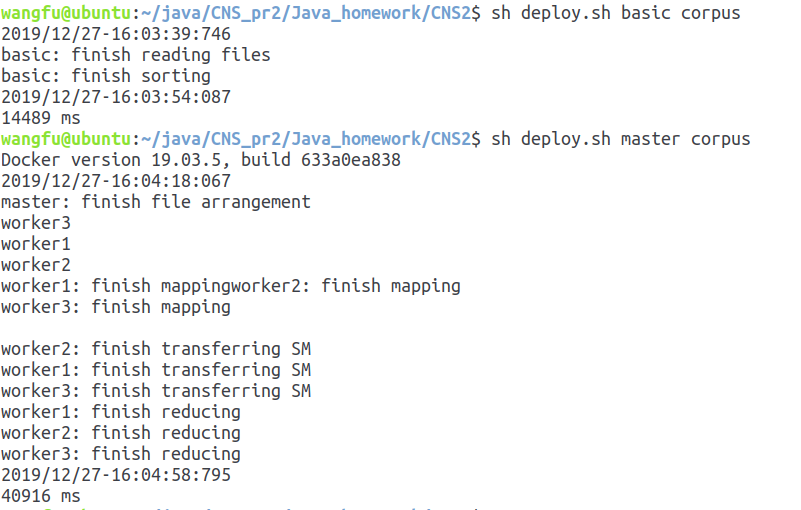
\includegraphics[width=12cm]{run}
		\end{center}
		\caption{Demo of build and run}
	\end{figure}

	\begin{figure}[h]
		\setlength{\abovecaptionskip}{-0.cm}
		
		\begin{center}
			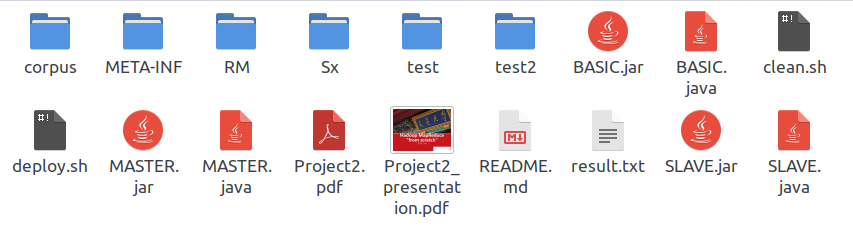
\includegraphics[width=12cm]{files}
		\end{center}
		\caption{Files used and generated by the program}
	\end{figure}

	\section{Experiment}
		\subsection{Comparison of two methods}
		\quad We have done the experiment for three files with a size of 117B, 8.2MB and 193.8MB respectively. The test results are shown as follows: 
		
		\begin{figure}[h]
			\setlength{\abovecaptionskip}{-0.cm}
			
			\begin{center}
				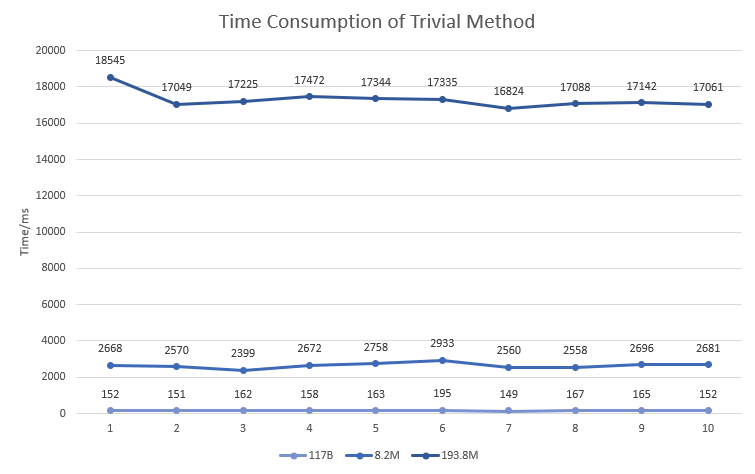
\includegraphics[width=12cm]{trivial_method}
			\end{center}
			\caption{Time consumption of Trivial method}
		\end{figure}
	
		\begin{figure}[H]
			\setlength{\abovecaptionskip}{-0.cm}
			
			\begin{center}
				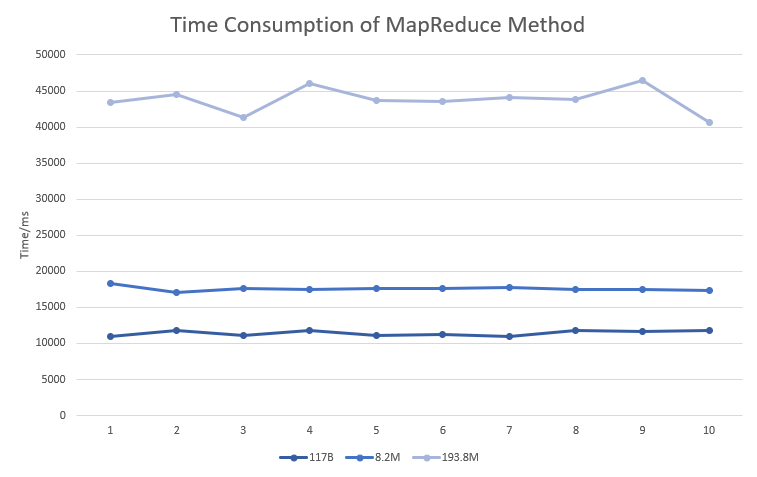
\includegraphics[width=12cm]{mapreduce_method}
			\end{center}
			\caption{Time consumption of MapReduce method}
		\end{figure}

	
		\quad The three curves of time consumption show that both of the two methods are stable for files with different sizes. As we can observe in the chart of performance, the bigger the file is, the more time these two methods consume. Theoretically, the MapReduce method should consume less time than the trivial method. However, in the experiment, we obtain the opposite result. After analyze and discussion, we give the following reasons: 

		
		\begin{itemize}
			
			\item 
			The reading, creation and transimission of the files cost too much time for MapReduce method. We can see that even with the smallest  file, MapReduce method  still needs more than 11 seconds in average. \\
			
			\item 
			We have done the work with docker on one computer where all the processes share the resources of one processor. If we use three computers to execute the slave programs, the result may be better.  \\
			
			\item 
			The input file is still not big enough to show the power of the MapReduce method. We can see that, with the increase of the file size, the time consumption of trivial method augments faster than that of MapReduce method. Hence, if the test file is large enough, for example, several GB, it is certain that the MapReduce method will cost less time. \\
			
			\item
			The operation system may use more than one cores or threads of the processor to run the trivial method. But as we generated three slaves on one computer, each slave has at most one core to use (the processor only has four cores). The available threads for each slave is less than that for the trivial process. \\
			
		\end{itemize}	

	
	\subsection{Improvements}
	
	To improve the performance of our MapReduce method, we can have some improvements in the algorithm as follows:
	
	\begin{itemize}
		
		\item 
		We can avoid reading the input file line by line and dividing it into three files. In reverse, it is possible to distribute the whole text files one by one, which can economize the time of reading files.  \\
		
		\item 
		In our program, we create three slaves. It is possible that with more slaves, the performance of MapReduce could be better.\\
		
		\item 
		For the mapping step, we divide the words by the first lettre "R" and "i". Maybe it is not the best choice, some of the slaves receive much more words than the others. We can try other choices to make the mapping more equal.\\
		
		\item 
		The last thing is to run the slave program on different computers and test with larger files.  \\
		
	\end{itemize}
	
	%% try special symbols
	\begin{comment}
		\begin{flushleft}
			
			$\bullet$ \ \textless special\textgreater ::= ”零” $\mid$ ”一” $\mid$ ”二” $\mid$ ” 三” $\mid$ ” 四” $\mid$ ” 五” $\mid$ ” 六” $\mid$ ” 七” $\mid$ ” 八” $\mid$ ” 九” $\mid$ ” 十” $\mid$ ” $\to$” \par
			
			$\bullet$ \ \textless a$\mid$b\textgreater  \par
			
		\end{flushleft}
	\end{comment}
				
	\begin{figure}[h]
		\setlength{\abovecaptionskip}{-0.cm}
			
		\begin{center}
			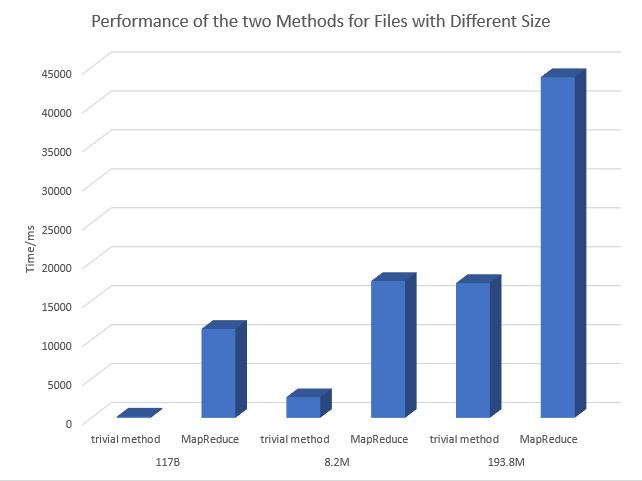
\includegraphics[width=12cm]{performance}
		\end{center}
		\caption{Performance of two methods for files with different sizes}
	\end{figure}

\end{document}